% !TEX root =  ./main.tex

\section{Encoding of RS in GT}\label{sec:RS2GTS}

Instead of BioResolve, we can alternatively use graph transformation to generate the underlying LTS of a given Reaction System, on the basis of a start graph (plus dedicated specialised type graph) obtained by transformation from the RS specification. What's more, we can analyse the outcome by building the \emph{occurrence graph} of a given trace, which contains all the rule occurrences and entity instances present in that trace --- anaogous, in fact, to the way a Petri net process captures a particular behaviour of a Petri Net. Moreover, if a trace leads to the state in which an undesirable entity is present (for instance, the $\anger$ entity in our toy example), we can also \emph{prune} the occurrence graph, again using graph transformation, to filter those rule occurrences and entity instances that directly contributed to the existence of the undesirable entity.

This gives rise to the tool chain depicted in \Cref{fig:chain}, the phases of which will be explained in some more detail in the remainder of this section.	

\begin{figure}
\centering
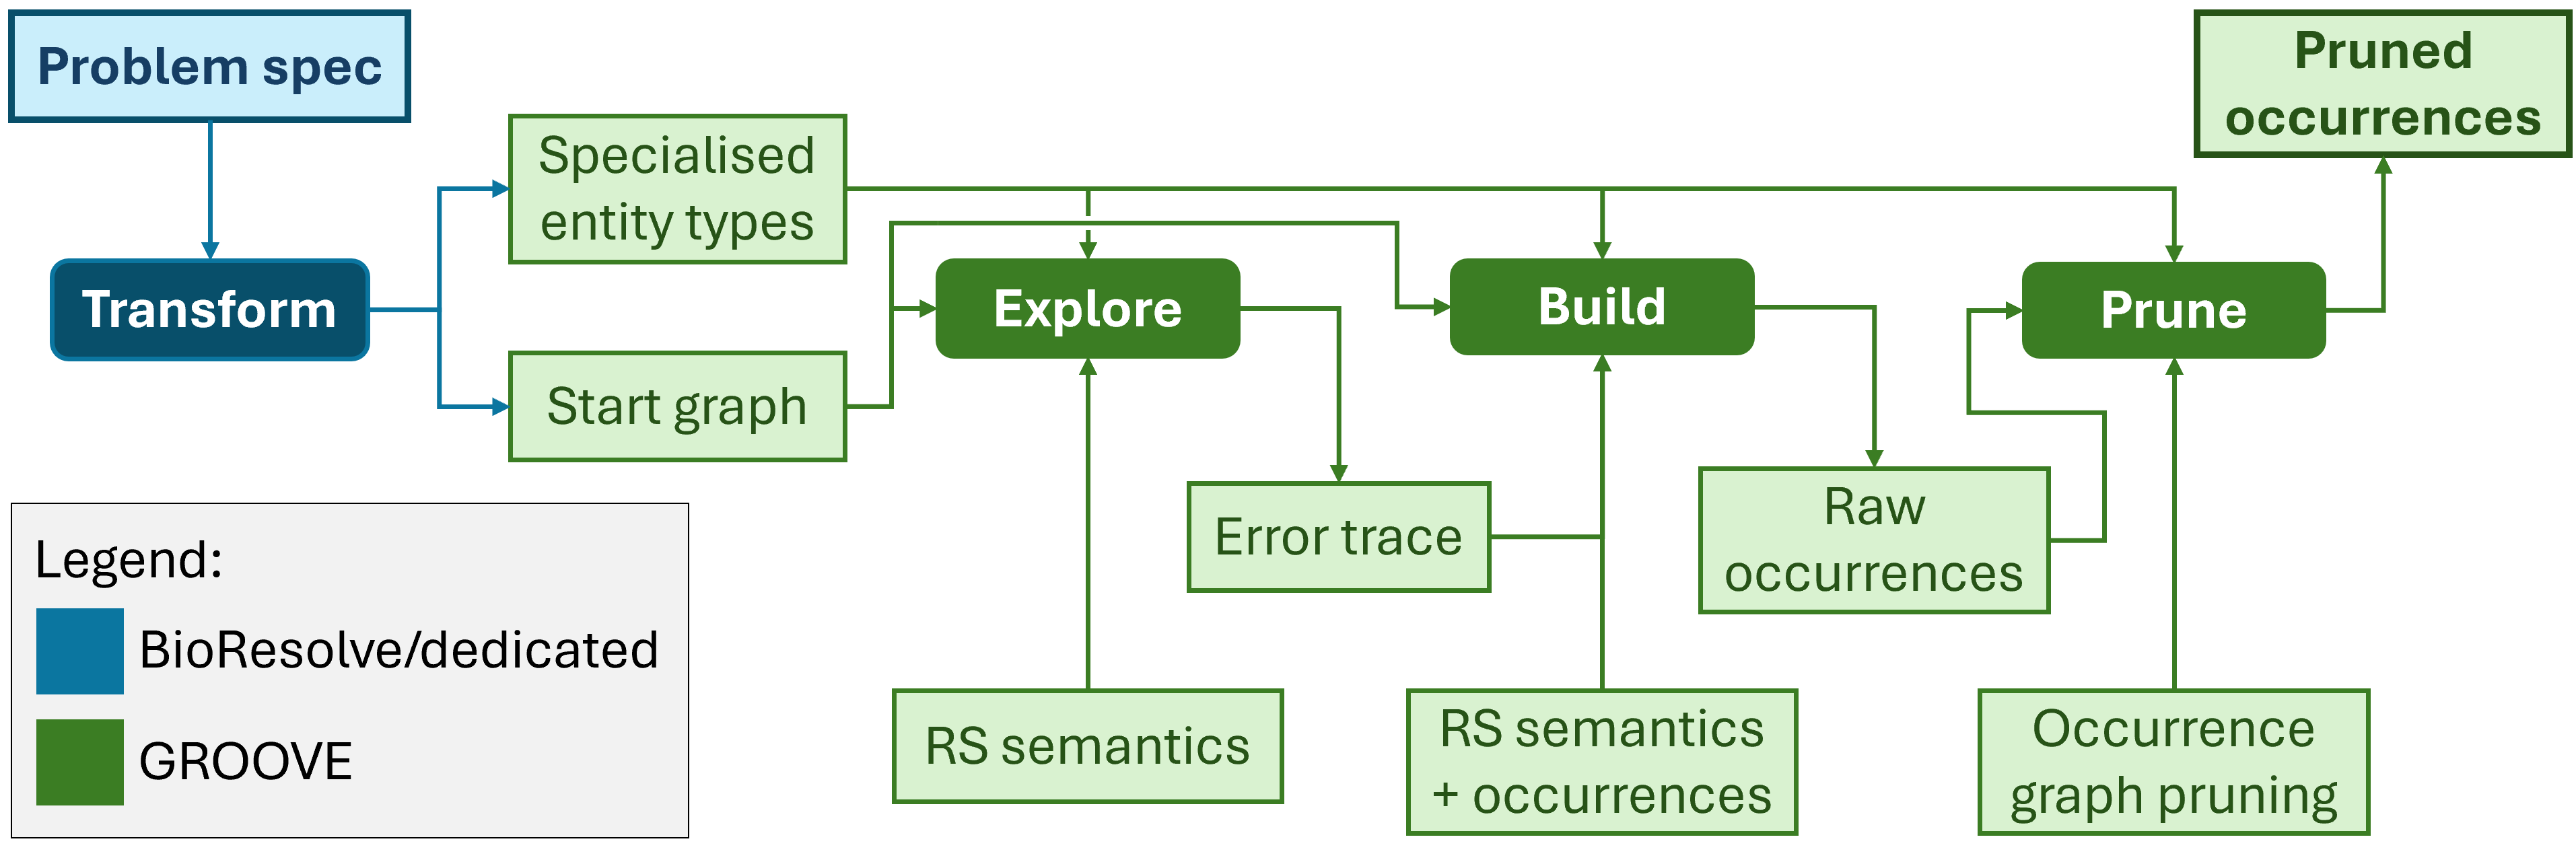
\includegraphics[scale=.25]{figs/chain}
\caption{Reaction System exploration and analysis using \GROOVE}
\label{fig:chain}
\end{figure}

\medskip\noindent\textbf{Transform.}
%
The first step is a text-to-model transformation from a problem specification in \BioResolve syntax into \GROOVE syntax. This produces two artifacts: firstly, an additional type graph, complementary to the one shown in \Cref{fig:core-type}, in which all entities in the problem at hand are provided with their own type (essentially for performance reasons: it speeds up the matching step of \GROOVE); and secondly (more importantly) a start graph in which the entire BioResolve system is encoded as suggested by \Cref{fig:core-type}. For the example system, the additional types as well as two fragments of the start graph are shown in \Cref{fig:toy}.

\begin{figure}
\centering
\subcaptionbox{Specialised entity types}{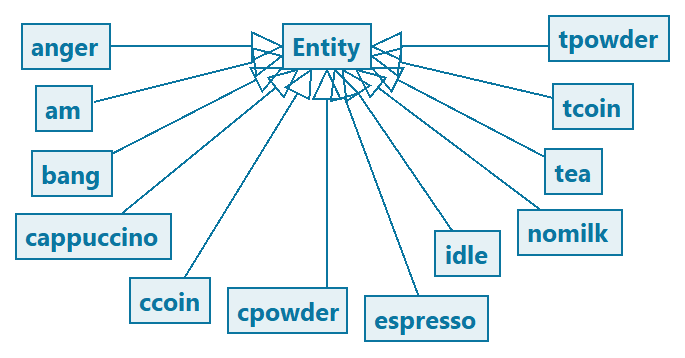
\includegraphics[scale=.2]{figs/toy-type}}
\subcaptionbox{Start graph fragment: Three of the reactions}{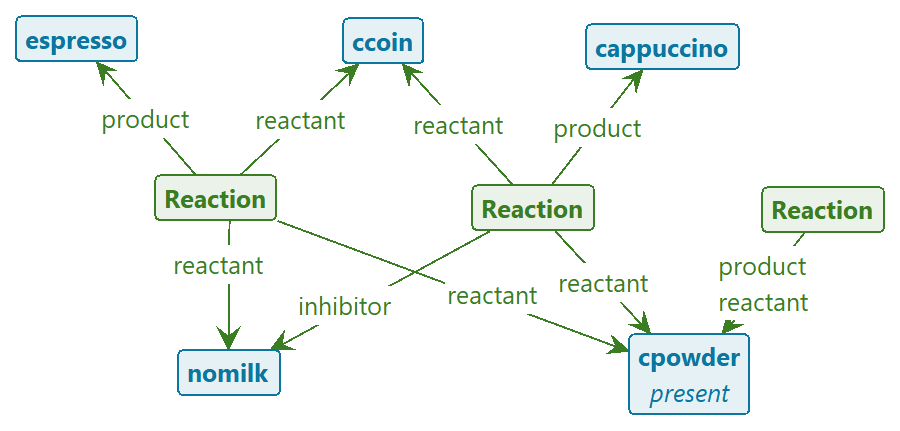
\includegraphics[scale=.2]{figs/toy-reactions}}
\subcaptionbox{Start graph fragment: The \textsf{Student} context process}{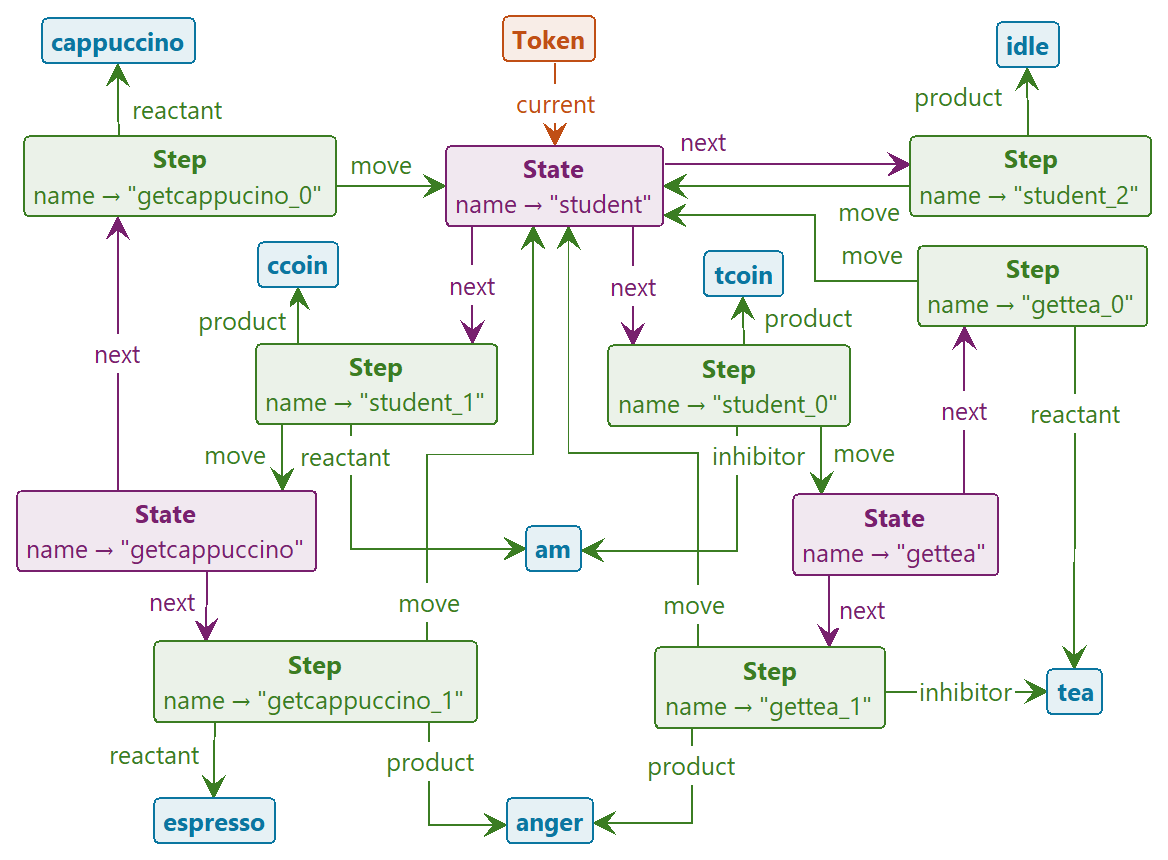
\includegraphics[scale=.2]{figs/toy-context-named}}
\caption{Graph representation of running example}
\label{fig:toy}
\end{figure}

\medskip\noindent\textbf{Explore.}
%
The reaction system semantics is encoded as a combination of two rules, \contextR and \reactR, which are scheduled to fire in alternation. \contextR encodes the simultaneous firing of all context processes (nondeterministically selecting an enabled \Step from every \State with a \Token), whereas \reactR encodes the (deterministic) simultaneous firing of all enabled \Reaction{}s, while simultaneously erasing all \Entity{}s that were not just produced. The production or erasure of an \Entity is encoded through the creation or deletion of a \present flag on a (persistent) \Entity node, \emph{not} by the creation or deletion of the node itself. In addition, to keep track of which nondeterministic choices were actually taken, the \contextR rule marks the \Step{}s that were selected with a \fired flag, which is subsequently erased by the reaction rule; a third rule called \firedR (actually a \emph{condition}, which in \GROOVE is a rule that does not modify the graph) checks for the occurrences of the \fired flag and so exposes the names of the \Rule{}s that have fired in the transition system.

\begin{figure}
\centering
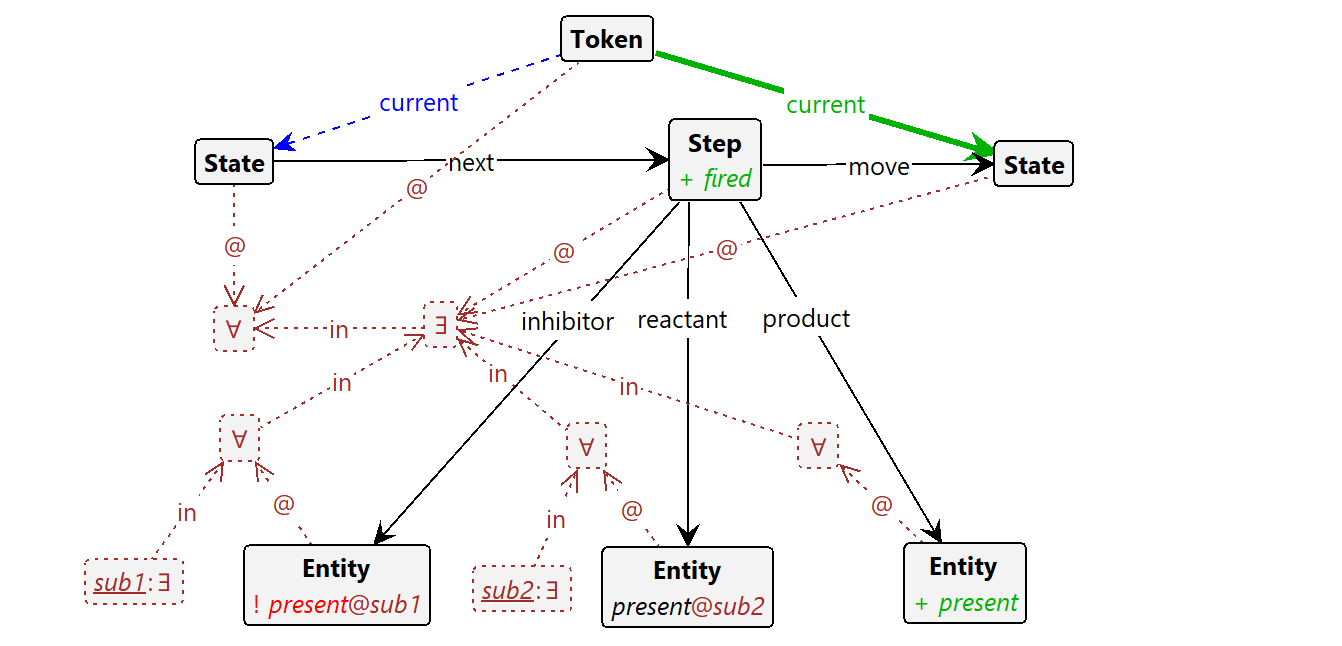
\includegraphics[scale=.2]{figs/context}
\caption{Rule for context firing}
\label{fig:context}
\end{figure}
%
\Cref{fig:context} shows the first (and most intricate) of these rules, viz.\ the one for the context firing. This is a quantified rule, which can be read as follows: \uline{For all} \State{}s with a \Token, \uline{there is} a \nextt{} \Step such that \uline{for all} \inhibitor{}s \uline{there is no} \present flag whereas \uline{for all} \reactant{}s \uline{there is} a \present flag; moreover, when the rule is applied, \uline{all} \product{}s of the selected \Step{}s receive a \present flag, the \Step{}s themselves receive a \fired flag, and all \Token{}s move to the successor \State{}s. Colour coding is used in the visual representation to distinguish the quantifier nodes $\forall$ and $\exists$ (purple), as well as the mandatory absence (red), deletion (blue) and creation (green) of edges and flags.\footnote{This colour coding is \GROOVE-specific and entirely separate from the problem-specific colouring of the graph nodes in Figures \ref{fig:core-type} and~\ref{fig:toy}; in fact, to avoid confusion, the problem-specific colouring is \emph{not} used in the rule view.}

\GROOVE can be set generate the entire state space, which is essentially the same as the one produced by BioResolve (see \Cref{fig:toylts}), but it can also be asked to search the for the first reachable state in which the \Forbidden entity appears, using breadth-first search. (In fact, the pattern for which \GROOVE searches is itself determined by a rule, which in this case merely tests for the presence of \Forbidden). When found, the trace to the undesirable state can be saved as a \emph{control program} that drives the next stage of \GROOVE exploration. In particular, besides the alternating application of the \contextR and \reactR rule --- the core of the Reaction System semantics --- this control program records the \firedR-applications that tell which \Step{}s have fired: this completely determines how the non-determinism in the context process has been resolved in order to arrive at the undesirable state. Here is the control program for our running example:

\begin{center}
\begin{lstlisting}[basicstyle=\sffamily\small,columns=fullflexible,xleftmargin=1cm]
context;
fired("student_2");
fired("refill_1");
react;
context;
fired("student_1");
fired("refill_0");
react;
context;
fired("refill_1");
fired("getcappuccino_1");
react;
\end{lstlisting}
\end{center}
%
Here \textsf{student\_2}, \textsf{student\_1} and \textsf{getcappucino\_1} are the \Step{}s of the \textsf{Student} process visualised in \Cref{fig:toy}; \textsf{refill\_1} and \textsf{refill\_0} are the steps of the \textsf{Refill} process given in \Cref{sec:student}.

\medskip\noindent\textbf{Build.}
%
The purpose of this phase is to build an occurrence graph that explains how \Forbidden was produced, by collecting its (transitive) dependencies. Concretely, we record the following dependencies:\todo{Refer to literature}
\begin{itemize}
\item From each non-initial \Entity instance to the \Rule occurrence of which it is the \product;
\item From each \Rule occurrence to all its reactant \Entity instances;
\item From each \Step occurrence to all directly preceding \Step occurrences.
\end{itemize}
%
Note that this is restricted to \emph{positive} dependencies.\todo{We could point out the modelling trick of using \espresso as a reactant of \anger, instead of \cappuccino as an inhibitor} The representation of negative dependencies is a research question in its own, and is outside the scope of this paper;\todo{Refer to literature} \Cref{fig:occur-type} shows the occurrence type graph. 

\begin{figure}
\centering
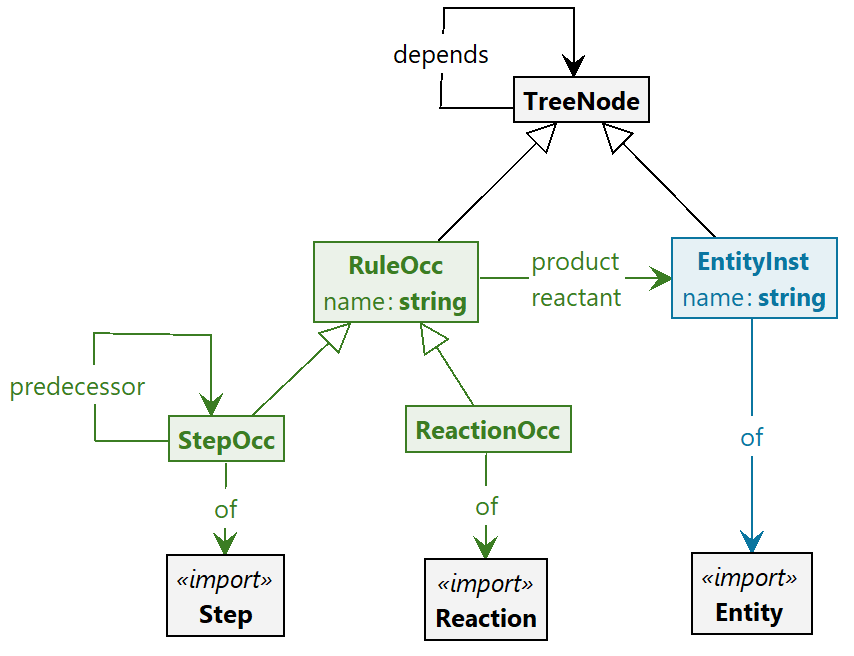
\includegraphics[scale=.2]{figs/occur-type}
\caption{Occurrence type graph}
\label{fig:occur-type}
\end{figure}

As indicated in \Cref{fig:chain}, the occurrence graph is produced by another \GROOVE rule system, using the same start graph but driven by the control program previously created in the explore phase, encoding (as we have seen) the trace to the undesirable state. The occurrence graph semantics consists of rules with the same names (\reactR, \contextR and \firedR), but different functionality: in particular, rather than manipulating \present flags, the \reactR rule now creates \RuleOcc- and \EntityInst-nodes together with their dependencies. This is a non-trivial procedure that in fact itself requires several successive stages. Though the details of these stages are not of sufficient interest to include in this paper, we want to point out that breaking down a single rule (\reactR, in this case) into multiple stages is opposed to the usual view, engrained in algebraic graph transformation, that a rule embodies a single, atomic change to a graph. This contradiction is solved by another feature of \GROOVE, namely \emph{recipes}. A recipe is a procedural control abstraction that has transactional semantics, and hence for the purpose of exploration acts just like an atomic rule; however, its body may consist of an arbitrary control (sub-)program. In the occurrence graph semantics, therefore, \reactR is actually not a rule but a recipe, defined as

\begin{center}
\begin{lstlisting}[basicstyle=\sffamily\small,columns=fullflexible,xleftmargin=1cm,keywords={recipe},literate={-}{-}1]
recipe react() {
  entities-age;
  react-produce;
  merge;
}
\end{lstlisting}
\end{center}
%
\medskip\noindent\textbf{Prune.}
%
Unfortunately, the occurrence graph built by the rule system described above is too large to be useful: it contains \emph{all} entities and rule occurrences produced by the trace, not just the dependencies of the undesired \Forbidden entity. Moreover, the entire start graph is also (still) present. Therefore, in a third phase, all redundant information is pruned. This is achieved by first marking all transitive backward dependencies of \Forbidden, and then removing all unmarked nodes. Since this is straightforward, and of no particular interest in the context of this paper, we omit the details of the \GROOVE rule system for this phase. Its outcome for our running example is shown in \Cref{fig:toy-pruned}.


\begin{figure}
\centering
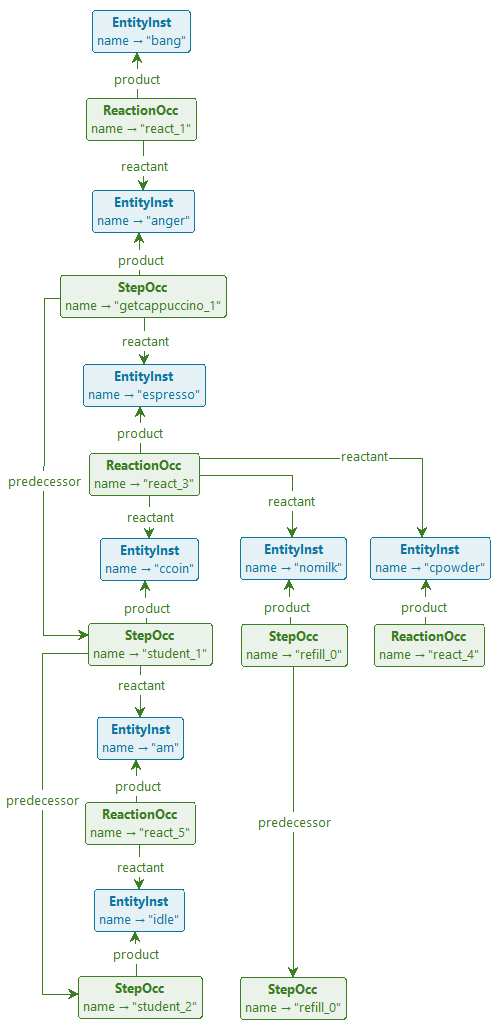
\includegraphics[width=\columnwidth]{figs/toy-pruned}
\caption{Pruned occurrence graph}
\label{fig:toy-pruned}
\end{figure}

The pruned occurrence graph visualises the causal effect chain already explained informally at the end of \Cref{sec:student}: the presence of a \ccoin, which itself depends on \am, combined with \cpowder and \nomilk causes the production of \espresso, after which the student produces \anger, which is \Forbidden.

\begin{comment}
\begin{quote}\it Notes:
\begin{itemize}
\item Rules for implementing RS semantics
\item Conversion of a trace to a control program
\item Using recipes in the occurrence graph building
\end{itemize}
\end{quote}
\end{comment}